\documentclass[utf8, xcolor, usenames,dvipsnames, aspectratio=169]{beamer}
\usepackage[english] {babel}
\usepackage[T1]      {fontenc}

\usepackage{amsmath, amsfonts, graphicx}
\usepackage{bibunits, tikz}
\usepackage{multirow}
\usepackage{float}


\usetheme{progressbar}

\setbeamersize
  {text margin left=1em, text margin right=1em}

\title
  [Contract Management Workflow]
  {Introduction of a Contract Management Workflow \centering at codecentric AG}

\author
  [Pia Erbrath]
  {Pia Erbrath (2300869)}

\date
  {Venlo, \today}

\institute
  {FHTenL Venlo}

\begin{document}

\maketitle

\begin{frame}{Overview}

  \tableofcontents

\end{frame}

\section{Introduction}
%\subsection{Assignment}
\begin{frame}{Assignment}
	\begin{itemize}
		\item Customer:
		\begin{enumerate}
			\item Wacom
			\item codecentric AG
		\end{enumerate}
		\item Creation/ Introducing Contract Management System
		\item Scope/Priority:
		\begin{enumerate}
			\item Electronically signing
			\item Archiving
			\item Creation
			\item Remembering
		\end{enumerate}
	\end{itemize}
\end{frame}

%\subsection{Time Planning}
\begin{frame}{Time Planning}
	\begin{table}
		\begin{tabular}{|p{0.5cm}|p{9cm}|p{1.5cm}|} \hline
			\textbf{\#} & \textbf{Phase} & \textbf{Week} \\ \hline
			1 & Project Planning & 1-6\\ \hline
			\color{BlueGreen} 2 & \color{BlueGreen} Analysis of the current situation and the requirements needed & \color{BlueGreen} 7-9\\  \hline
			3 & Designing of a new workflow & 10-12 \\ \hline
			4 & Implementation and testing of the workflow based on the defined scope & 13-18 \\ \hline
			5 & Finalize bachelor thesis & 23,24 \\ \hline
		\end{tabular}
		\caption{Time Planning}
	\end{table}
\end{frame}

\section{Analysis Current Situation}
%\subsection{Business Processes}
\begin{frame}{Business Process}
	\begin{figure}[t]
		\centering
		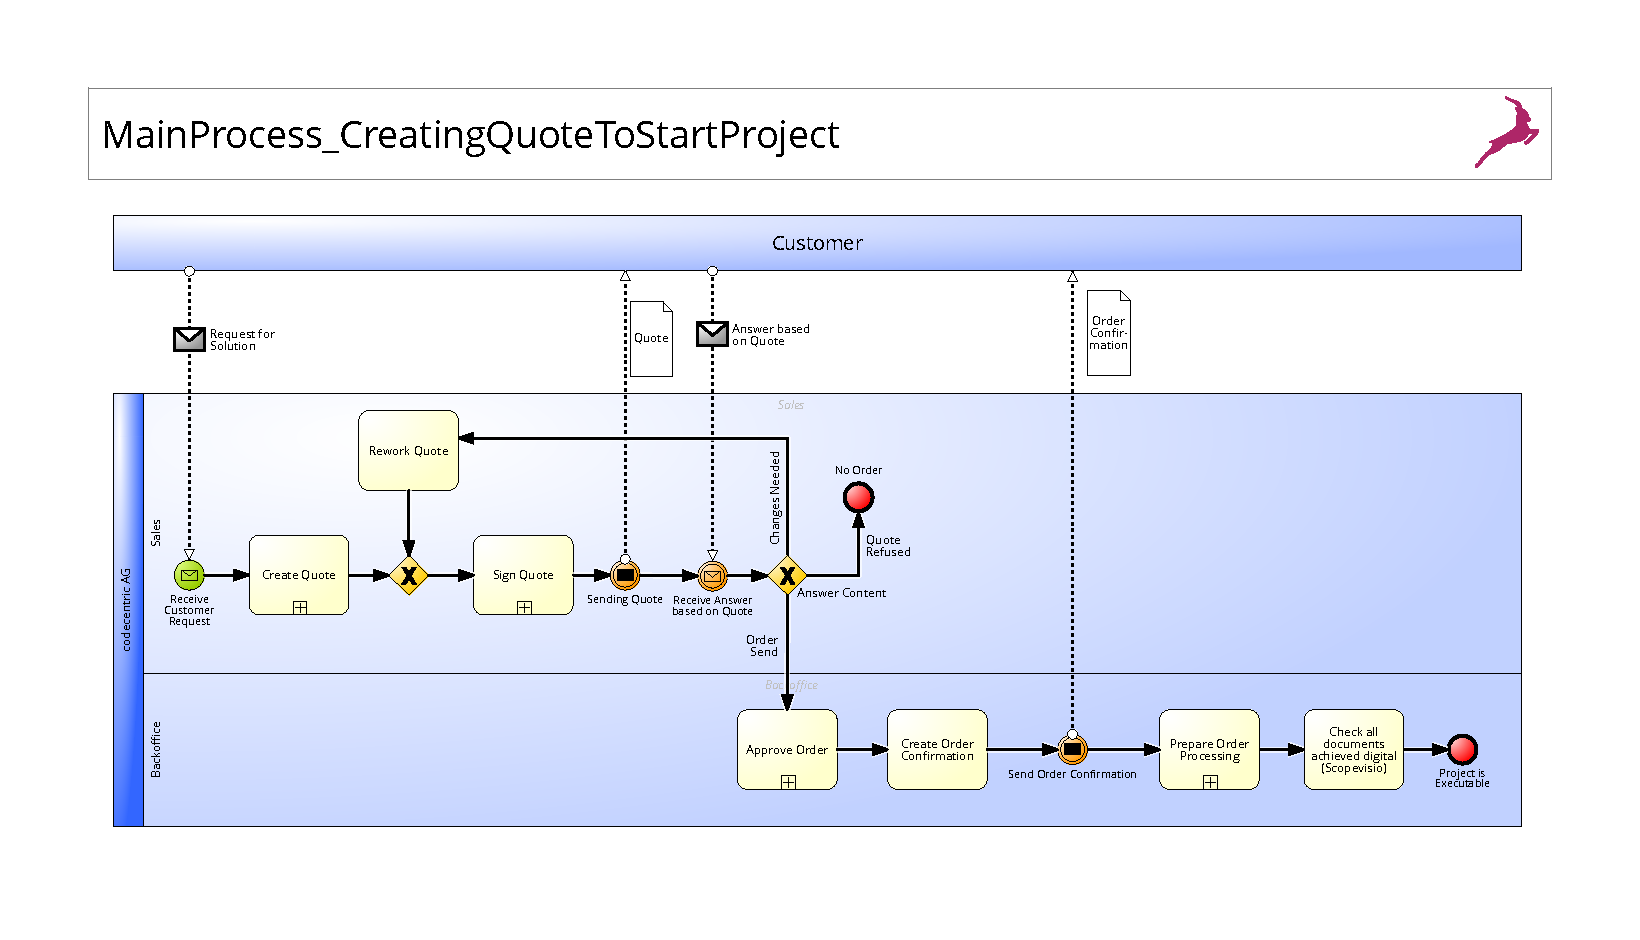
\includegraphics[width=0.9\textwidth, height=0.85\textheight]{./images/0_main}
		\caption{Main Process Quote}
	\end{figure}
\end{frame}

\begin{frame}{Sub Processes}
	\begin{figure}[t]
		\centering
		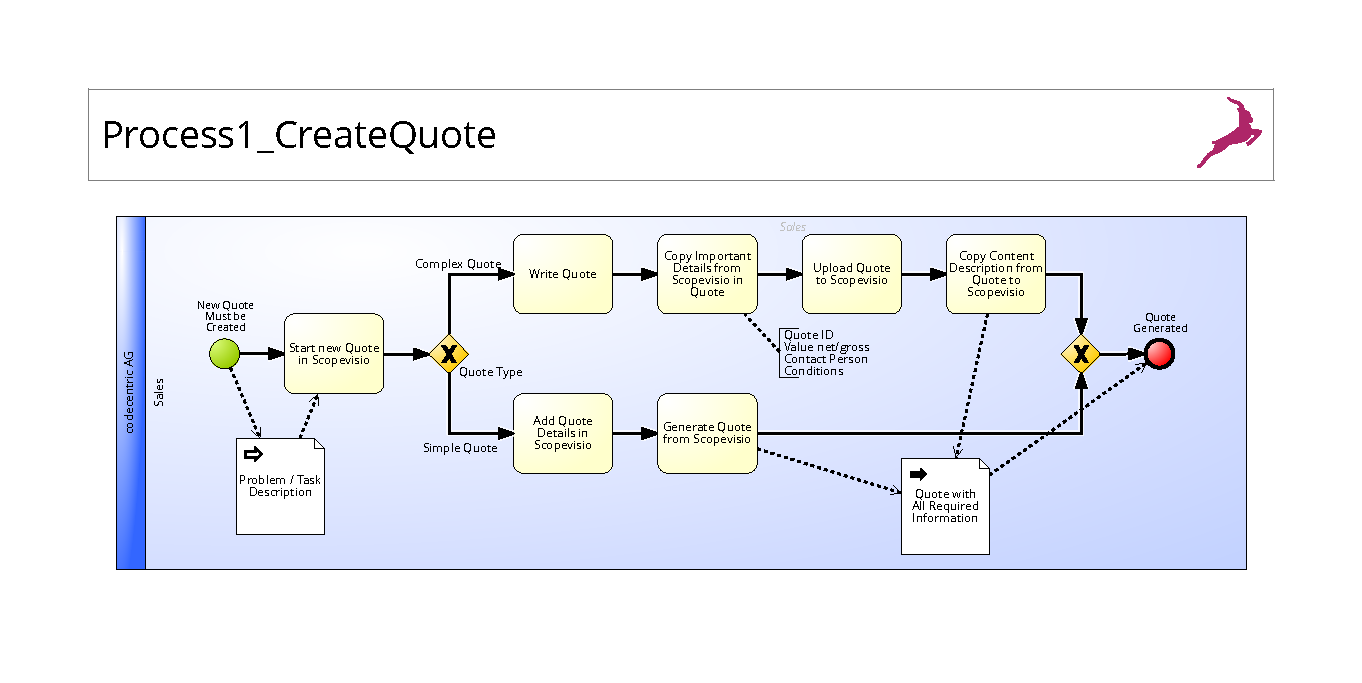
\includegraphics[height=0.9\textheight]{./images/0-1_createQuote}
		\caption{Sub Process Quote Creation}
	\end{figure}
\end{frame}

\begin{frame}{Sub Processes}
	\begin{figure}[t]
		\centering
%		height=\dimexpr11\textheight/16\relax
		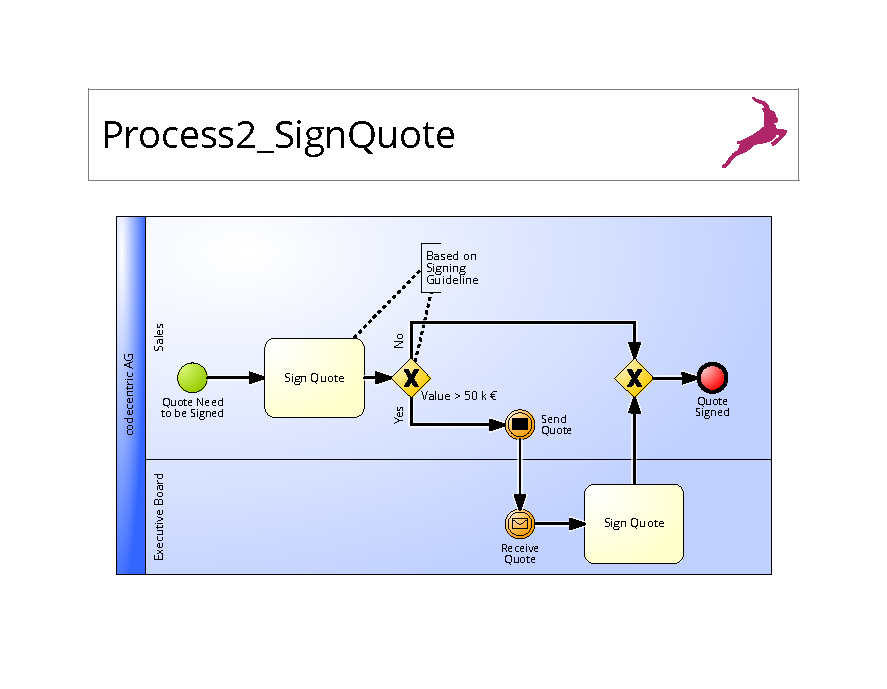
\includegraphics[height=0.9\textheight]{./images/0-2_signQuote}
		\caption{Sub Process Signing Quote}
	\end{figure}
\end{frame}

%\subsection{Problems}
\begin{frame}{Problems}
	\begin{itemize}
		\item To many manual steps (Signing, Archiving)		
		\item Incorrect signing of documents 
		\item Signing guideline outdated
		\item Document creation
	\end{itemize}
\end{frame}

\section{Conditions New Process}
%\subsection{Aims}
\begin{frame}{Aims}
	\begin{enumerate}
		\item Create standard workflow
		\item Automate achieving
		\item Reduce manual work (creation \& signing)
		\item Paperless office
	\end{enumerate}
\end{frame}

%\subsection{Requirements}
\begin{frame}{Requirements}
	\begin{itemize}
		\item Standard processes
		\item Accepted documents format
		\item Transparency \& Fulfillment signing guideline
		\item Legal standard
	\end{itemize}
\end{frame}

\section{Research}
%\subsection{Electronic Signature}
\begin{frame}{Electronic Signature}
	\begin{itemize}
		\item eIDAS 
		\item 3 Types
		\begin{enumerate}
			\item Simple electronic signature
			\item Advanced electronic signature
			\item Qualified electronic signature
		\end{enumerate}
		\item Biometric signature 
	\end{itemize}
\end{frame}

%\subsection{Tool Signing Documents Electronically}
%\begin{frame}{Tool Signing Documents Electronically}
%	content...
%\end{frame}

\section{Conclusion}
%\subsection{Reflection}
\begin{frame}{Reflection}
	\begin{enumerate}
		\item What went good:
		\begin{itemize}
			\item Cooperation with employees
			\item Time planning till now
		\end{itemize} 
		\item Possible Problems:
		\begin{itemize}
			\item New ERP system
		\end{itemize}
	\end{enumerate}
\end{frame}

%\subsection{Lookup}
\begin{frame}{Lookout}
	\begin{itemize}
		\item Finalize research about electronic singing tool
		\item Design new workflow
		\item Implement signing step of new workflow
	\end{itemize}
\end{frame}

\begin{frame}{Conclusion}
	\begin{itemize}
		\item A lot of problems, not all can be solved
		\item The implementation maybe prototype $\rightarrow$ new ERP system / old ERP
		\item Properly in time
	\end{itemize}
\end{frame}

\begin{frame}
	\begin{center}
		{\Huge Questions left?}
	\end{center}
\end{frame}

\end{document}
